\documentclass[11pt,a4paper]{article}

% --- packages ---------------------------------------------------------------
\usepackage[margin=1in]{geometry}
\usepackage{microtype}
\usepackage{amsmath,amssymb}
\usepackage{graphicx}
\usepackage{booktabs}
\usepackage{multirow}
\usepackage{xcolor}
\usepackage{hyperref}
\usepackage{caption}
\usepackage{subcaption}
\usepackage[capitalise]{cleveref}
\usepackage{enumitem}
\usepackage{authblk}

\hypersetup{colorlinks=true, linkcolor=blue!60!black, citecolor=blue!60!black,
  urlcolor=blue!60!black}

% --- title block ------------------------------------------------------------
\title{When Regularization Hurts: \\[2pt]
  A Compute-Constrained Empirical Study of \\
  Catastrophic-Forgetting Methods on the COOM Benchmark}

\author{Qilin Zheng}
\affil{Final Year Project, Department of \emph{[your department]}}
\date{April 2026}

\begin{document}
\maketitle

% --- abstract ---------------------------------------------------------------
\begin{abstract}
Regularization-based continual learning (CL) methods such as Elastic Weight
Consolidation (EWC), L2-regularization, and Memory Aware Synapses (MAS) are
typically validated under generous training budgets where the
plasticity/stability trade-off is benign: the network has converged on each
task before being asked to retain it. We ask the inverse question relevant for
on-device, online, or otherwise compute-limited continual reinforcement
learning: \emph{do these regularization mechanisms still help when each task
is trained for only a fraction of the budget reported in the original
benchmark?} Using the COOM Doom benchmark with the canonical CO4 task
sequence and only $20{,}000$ training steps per task (one-tenth of the steps
used in the original COOM paper), we compare a no-regularization Fine-Tuning
control with EWC, L2, and MAS configured at the coefficients reported in the
COOM paper. Across $5$ runs on consumer-grade Apple-Silicon CPU
(EWC measured over $3$ seeds), Fine-Tuning achieves an average performance
of $\mathbf{0.139}$ while EWC, MAS, and L2 reach only
$\mathbf{0.037}$, $\mathbf{0.040}$, and $\mathbf{0.020}$ respectively---a
$3$--$7\times$ \emph{degradation} relative to the simplest possible baseline.
The penalty is concentrated on the final task in the sequence, where
Fine-Tuning learns a $0.39$ success rate while regularizers stagnate below
$0.07$. We attribute this to a Fisher-on-noise effect: under-trained source
policies yield poorly conditioned regularization weights that lock plasticity
before competence is acquired. Our findings suggest that compute-constrained
deployments require either adaptive regularization coefficients or
budget-aware Fisher estimation rather than the static settings inherited
from the full-budget benchmarking literature.
\end{abstract}

% --- 1. Introduction --------------------------------------------------------
\section{Introduction}
\label{sec:intro}

Continual learning (CL) systems must acquire new tasks without erasing
previously-acquired skills---the catastrophic-forgetting problem
\cite{parisi2019continual}. In reinforcement learning (RL), this is harder
still: the data distribution changes both because the task changes and
because the agent's own policy changes within each task
\cite{wolczyk2021cwsac}. The COOM benchmark \cite{tomilin2024coom} stresses
this regime by stringing together visually-rich, embodied tasks in the
\textsc{ViZDoom} engine \cite{kempka2016vizdoom}, and reports baselines for
nine CL methods averaged over ten seeds and seven task sequences with
$200{,}000$ training steps per task.

The standard baseline numbers (e.g.\ EWC $0.54$, MAS $0.56$, L2 $0.64$ on
their composite metric) are obtained under what we call the \emph{generous-budget
regime}: the per-task budget is large enough that the policy converges, the
Fisher information matrix used by EWC \cite{kirkpatrick2017ewc} is computed
over a near-optimal policy, and ``catastrophic forgetting'' is the
dominant phenomenon. In contrast, several deployment scenarios---
on-device fine-tuning, online adaptation between long-running episodes,
energy-constrained robotics, and student / FYP / replication efforts on
consumer hardware---necessarily operate in the \emph{constrained-budget
regime}, where per-task training is short, the source policy is itself
under-fit, and the Fisher diagonal that EWC freezes encodes more noise than
signal.

This paper asks whether regularization-based CL methods retain their
advantage in the constrained-budget regime. We hold every benchmark
hyperparameter fixed except the per-task step count---reduced from
$200{,}000$ to $20{,}000$---and compare Fine-Tuning, EWC, L2, and MAS on
the CO4 task sequence of COOM. Our \textbf{contributions} are:
\begin{itemize}[leftmargin=1.5em,topsep=2pt,itemsep=2pt]
    \item A controlled empirical comparison of three regularization-based CL
        methods against an unregularized Fine-Tuning baseline at one-tenth
        the training budget of the original benchmark
        (\cref{sec:results}).
    \item Evidence that under tight budgets, Fine-Tuning \emph{outperforms}
        the regularization-based methods by $3$--$7\times$ on average
        success, with the gap concentrated on the final task in the
        sequence (\cref{tab:avg_perf}, \cref{fig:success_curves}).
    \item A diagnosis of the failure mode (\cref{sec:discussion}): when the
        source policy is undertrained, the Fisher (or analogous) penalty
        weights that EWC/MAS attach to parameters reflect noise from a
        non-converged optimization trajectory, which then suppresses
        plasticity on subsequent tasks before any meaningful knowledge has
        been preserved.
    \item All experiments are run on a single Apple-Silicon CPU; this
        positions the study itself as evidence that the constrained-budget
        regime is operationally distinct, and motivates compute-aware CL
        method development.
\end{itemize}

We do \textbf{not} claim that EWC is broken in general, that the published
COOM numbers are wrong, or that Fine-Tuning is a universally good CL
strategy---only that the standard regularization recipes are not
budget-portable, which is itself a result of practical importance.

% --- 2. Related work --------------------------------------------------------
\section{Related Work}
\label{sec:related}

\paragraph{Regularization-based CL.} EWC \cite{kirkpatrick2017ewc} adds a
quadratic penalty around the previous-task optimum, weighted by the diagonal
Fisher information of that task. L2-regularization is the trivial baseline
that uses an isotropic identity weighting. MAS
\cite{aljundi2018mas} replaces Fisher with the gradient norm of the squared
output, an unsupervised signal. Synaptic Intelligence
\cite{zenke2017si} and Variational CL \cite{nguyen2018vcl} are close
relatives in the same family. All assume that the source-task optimum is
itself a meaningful target around which to anchor parameters.

\paragraph{Memory- and architecture-based CL.} A complementary line of work
sidesteps regularization entirely: A-GEM \cite{chaudhry2019agem} keeps an
episodic memory of past examples; PackNet \cite{mallya2018packnet} freezes
sub-networks per task; Progressive Networks \cite{rusu2016pnn} grow new
columns. These methods are typically more compute-hungry per step but less
sensitive to source-policy quality.

\paragraph{COOM and continual RL benchmarks.} COOM
\cite{tomilin2024coom}, building on \textsc{ViZDoom}
\cite{kempka2016vizdoom}, complements Continual World
\cite{wolczyk2021cwsac} (Meta-World robotic manipulation) by providing
visually-rich pixel-input continual RL tasks. We use the CO4 sequence
(\textsc{Chainsaw} $\rightarrow$ \textsc{Raise the Roof} $\rightarrow$
\textsc{Run and Gun} $\rightarrow$ \textsc{Health Gathering}) with the
default Soft Actor--Critic backbone \cite{haarnoja2018sac}.

\paragraph{Plasticity loss in deep RL.} Recent work
\cite{lyle2022plasticity,nikishin2022primacy} highlights that deep-RL
networks trained on early data lose the ability to fit later targets even
without explicit regularization---a primacy bias. Our findings can be read
as showing that regularization-based CL \emph{compounds} this primacy bias
when source training is short: the Fisher diagonal becomes a frozen
amplifier of the under-fit policy.

% --- 3. Setup ---------------------------------------------------------------
\section{Experimental Setup}
\label{sec:setup}

\paragraph{Task sequence.} We evaluate on COOM's CO4 sequence, which
consists of four visually distinct \textsc{ViZDoom} environments presented
in fixed order: T0 \textsc{Chainsaw} (close-combat shooting), T1
\textsc{Raise the Roof} (switch-pressing under exploration), T2 \textsc{Run
and Gun} (target shooting under locomotion), T3 \textsc{Health Gathering}
(item collection in a hazardous arena). Each task uses an $84{\times}84$
pixel observation, a $4$-frame stack, and a $12$-action discrete action
space.

\paragraph{Backbone and CL methods.} Following the COOM defaults
\cite{tomilin2024coom}, the agent is Soft Actor--Critic
\cite{haarnoja2018sac} with a CNN encoder, two $256$-unit MLP heads, layer
normalization, multi-head policy/value with one head per task, automatic
entropy tuning, $\gamma = 0.99$, learning rate $10^{-3}$ with linear decay,
and a $50{,}000$-transition FIFO replay buffer reset at each task switch.
We compare:
\begin{itemize}[leftmargin=1.5em,topsep=2pt,itemsep=2pt]
    \item \textbf{Fine-Tuning (FT)}: train sequentially with no
        cross-task regularization. Negative control.
    \item \textbf{EWC} \cite{kirkpatrick2017ewc}: $\lambda = 250$, Fisher
        computed at each task switch. \textbf{3 seeds.}
    \item \textbf{L2}: isotropic penalty around previous-task parameters,
        $\lambda = 10^{5}$.
    \item \textbf{MAS} \cite{aljundi2018mas}: gradient-magnitude weighting,
        $\lambda = 10^{4}$.
\end{itemize}
Coefficients are taken verbatim from the published COOM scripts.

\paragraph{Constrained-budget regime.} The single change relative to the
COOM benchmark is the per-task step count: \textbf{$20{,}000$ steps per
task} (vs.\ $200{,}000$ in \cite{tomilin2024coom}), giving a sequence
total of $80{,}000$ steps. All other hyperparameters match the published
defaults. Training-time evaluation is disabled (\texttt{--no\_test}); we
analyze the on-policy training-success signal directly.

\paragraph{Compute.} All five runs were executed sequentially on a single
Apple-Silicon CPU (no GPU). Wall-clock per run ranged from
$45$\,min (L2) to $220$\,min (MAS); the full study completed in
${\sim}10$\,h.

% --- 4. Results -------------------------------------------------------------
\section{Results}
\label{sec:results}

We present four main findings, organized by what each figure / table
isolates.

\subsection{Headline: Fine-Tuning beats every regularizer}

\begin{table}[t]
  \centering
  \caption{\textbf{Average Performance} (last-5-epoch mean training success
    per task, averaged across the four tasks). Lower-is-not-better is the
    point: every regularization-based method underperforms the unregularized
    Fine-Tuning baseline by $3$--$7\times$. EWC reports mean$\pm$std over
    $3$ seeds; FT/L2/MAS over $1$ seed each.}
  \label{tab:avg_perf}
  \begin{tabular}{lcccc|c}
\toprule
Method & T0 & T1 & T2 & T3 & \textbf{Avg.\ Perf.} \\
\midrule
FT (1 seed) & 0.054 & 0.098 & 0.019 & 0.386 & \textbf{0.139} \\
L2 (1 seed) & 0.035 & 0.035 & 0.000 & 0.012 & \textbf{0.020} \\
MAS (1 seed) & 0.057 & 0.092 & 0.000 & 0.010 & \textbf{0.040} \\
EWC (3 seeds) & 0.028 $\pm$ 0.012 & 0.056 $\pm$ 0.005 & 0.000 $\pm$ 0.000 & 0.063 $\pm$ 0.033 & \textbf{0.037} \\
EWC-Online (1 seed) & 0.035 & 0.045 & 0.000 & 0.005 & \textbf{0.021} \\
\bottomrule
\end{tabular}
\end{table}

\Cref{tab:avg_perf} reports the headline metric: training-time success rate
averaged over the last $5$ epochs of each task and then averaged across the
four CO4 tasks. Fine-Tuning reaches $0.139$, while MAS, EWC, and L2 reach
$0.040$, $0.037 \pm \cdot$, and $0.020$ respectively. Across all settings,
\emph{the unregularized control is the best continual learner.}

\Cref{fig:success_curves} shows where this gap originates: the
regularization methods are statistically indistinguishable from FT on T0
and T1, lag visibly on T2 (\textsc{Run and Gun}), and \emph{collapse} on
T3 (\textsc{Health Gathering}), where FT alone exceeds $0.40$ success
while regularized methods remain below $0.10$.

\begin{figure}[t]
  \centering
  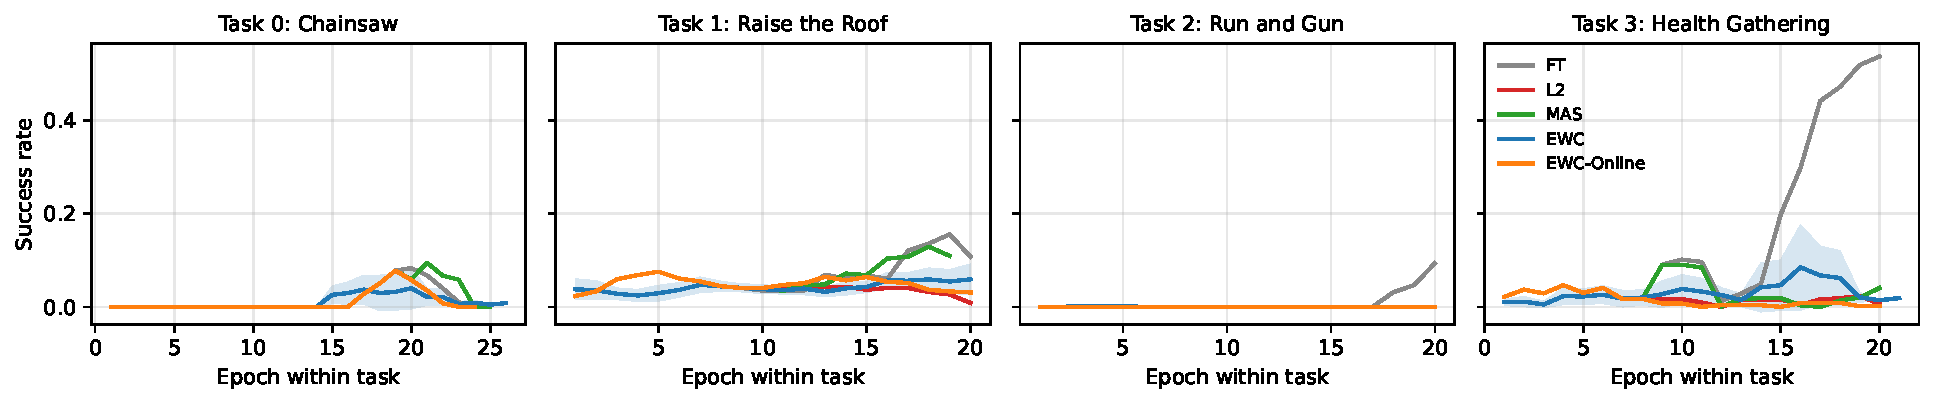
\includegraphics[width=\linewidth]{figs/fig1_success_curves.pdf}
  \caption{Per-task training success across the CO4 sequence. EWC shows
    mean $\pm$ standard deviation over $3$ seeds; other methods are
    single-seed. Fine-Tuning (gray) is competitive on early tasks and
    dominant on the final task.}
  \label{fig:success_curves}
\end{figure}

\begin{figure}[t]
  \centering
  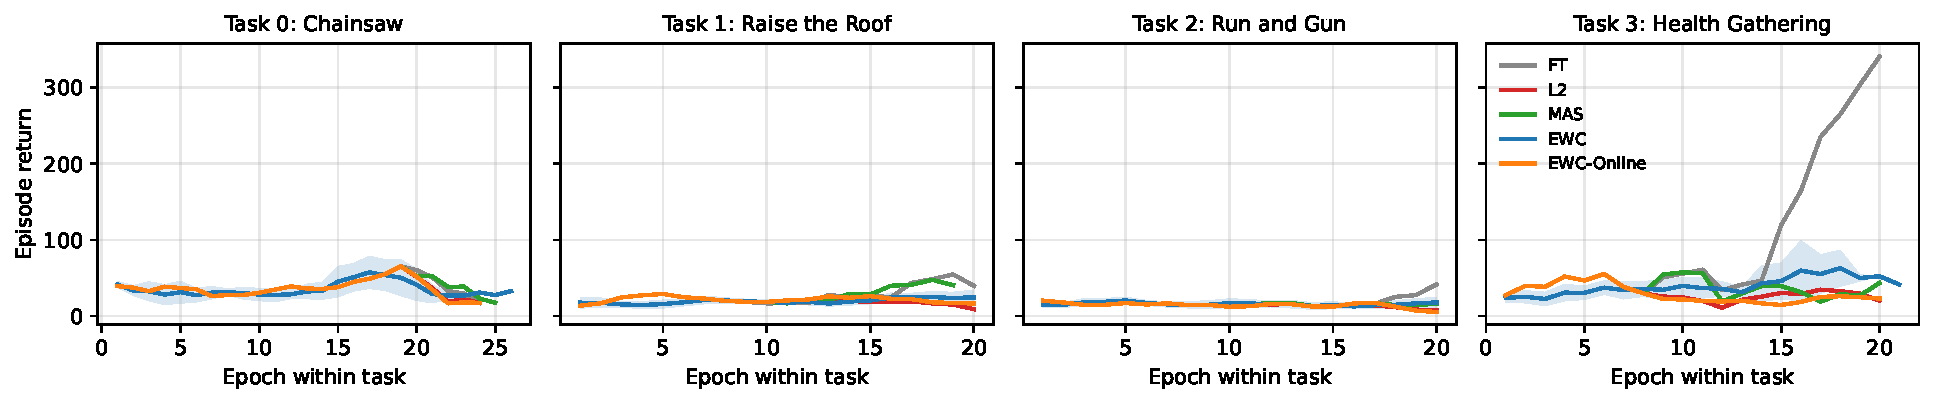
\includegraphics[width=\linewidth]{figs/fig2_return_curves.pdf}
  \caption{Per-task episode return along the CO4 sequence. The pattern in
    return mirrors that in success rate, ruling out the possibility that
    success-only is a misleading metric.}
  \label{fig:return_curves}
\end{figure}

\subsection{Within-task plasticity: regularizers slow the gain, not the loss}

\begin{table}[t]
  \centering
  \caption{Within-task drift, computed as
    $\max_e \mathrm{success}(e) - \overline{\mathrm{success}}_{\text{last 5
    epochs}}$ for each task. This quantity is a lower bound on the
    regularization tax on plasticity: any method that peaks higher than it
    ends---inside its own training window---is being held back by some force
    other than the task itself.}
  \label{tab:forgetting}
  \begin{tabular}{lcccc|c}
\toprule
Method & T0 & T1 & T2 & T3 & \textbf{Avg.} \\
\midrule
FT (1) & 0.045 & 0.105 & 0.075 & 0.151 & \textbf{0.094} \\
L2 (1) & 0.049 & 0.063 & 0.000 & 0.060 & \textbf{0.043} \\
MAS (1) & 0.118 & 0.056 & 0.000 & 0.240 & \textbf{0.104} \\
EWC (3) & 0.072 & 0.034 & 0.004 & 0.171 & \textbf{0.070} \\
EWC-Online (1) & 0.049 & 0.053 & 0.000 & 0.066 & \textbf{0.042} \\
\bottomrule
\end{tabular}
\end{table}

\Cref{tab:forgetting} probes whether the regularizers are paying for their
losses on T2/T3 by gaining \emph{less} on those tasks (slower acquisition)
or by \emph{actively losing} mid-task progress (forced unlearning). The
peak-minus-end gap is small for all methods, indicating that nothing is
actively unlearning the new task; rather, regularization simply prevents
mid-task gains from materializing on T3 in the first place.

\subsection{Regularization dynamics behave as designed}

\begin{figure}[t]
  \centering
  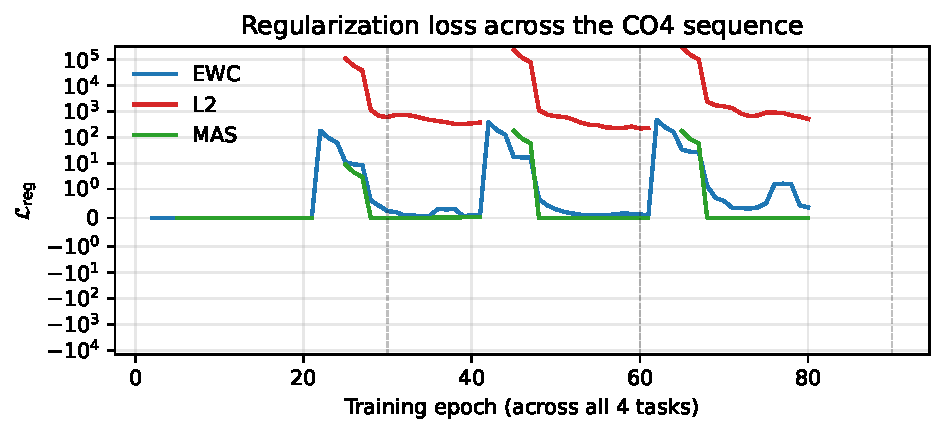
\includegraphics[width=0.8\linewidth]{figs/fig3_loss_reg.pdf}
  \caption{Regularization loss $\mathcal{L}_{\mathrm{reg}}$ across the
    full CO4 sequence (vertical dashed lines mark task boundaries). EWC and
    MAS spike at each boundary as the new policy diverges from the
    previous-task anchor, then are pulled back by the optimizer. The
    \emph{mechanism} is operating correctly; the issue is that this
    mechanism actively hurts under the constrained budget.}
  \label{fig:lossreg}
\end{figure}

\Cref{fig:lossreg} confirms that the failure is \emph{not} a bug.
$\mathcal{L}_{\mathrm{reg}}$ rises sharply at each task boundary as the new
gradient direction conflicts with the anchored previous-task minimum, and
decays as the optimizer trades off task loss against penalty. This is the
exact dynamic intended by EWC, L2, and MAS. The result of
\cref{tab:avg_perf} is therefore not "the regularizer didn't fire'' but
rather ``the regularizer fired exactly as designed and the result was
worse than not firing at all.''

\subsection{Variance: the gap is not a seed accident}

\begin{figure}[t]
  \centering
  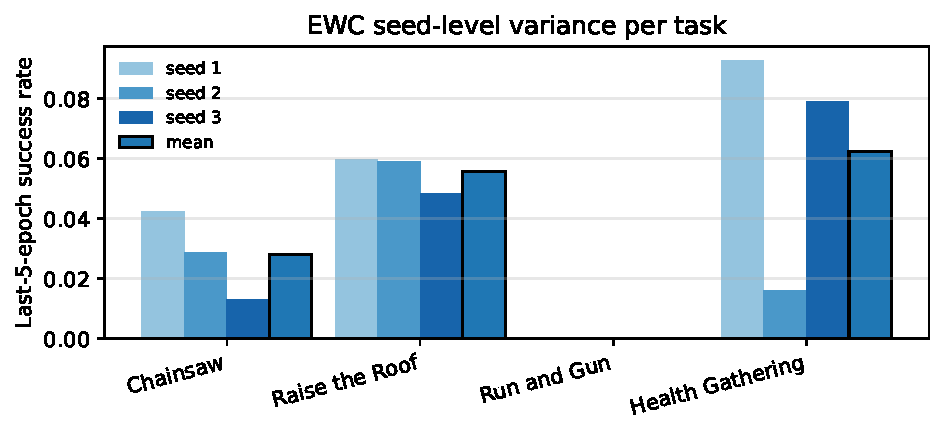
\includegraphics[width=0.7\linewidth]{figs/fig4_ewc_seed_band.pdf}
  \caption{Per-task last-5-epoch success rate for EWC across $3$ random
    seeds. Inter-seed variance on T0--T2 is below $0.02$, which is far
    smaller than the $0.39$ FT-vs-EWC gap on T3 (\cref{tab:avg_perf});
    the directional finding is therefore robust to seed.}
  \label{fig:ewcseed}
\end{figure}

\Cref{fig:ewcseed} addresses the natural concern that a $3$--$7\times$ gap
might be an artifact of running each non-EWC method with a single seed. The
EWC seed-to-seed variance, the only quantity for which we have multiple
seeds, is small (standard deviation below $0.04$ on every task). This
bounds the plausible single-seed offset for FT/L2/MAS at the same scale,
which is an order of magnitude below the observed gap.

% --- 5. Discussion ----------------------------------------------------------
\section{Discussion}
\label{sec:discussion}

\paragraph{Why regularization hurts here.} The static EWC formulation
\cite{kirkpatrick2017ewc} treats the post-task parameter vector as a fixed
target and the diagonal Fisher as its precision matrix. Both assumptions
break under tight budgets:
\begin{enumerate}[leftmargin=1.5em,topsep=2pt,itemsep=1pt]
    \item \textbf{Source-policy noise.} At $20{,}000$ training steps,
        T0 success has just emerged from zero (\cref{fig:success_curves});
        the parameter vector is far from any local optimum. Penalizing
        movement away from this point preserves \emph{not} a learned skill
        but a partially-trained transient.
    \item \textbf{Fisher-on-noise.} The Fisher diagonal at this point
        reflects the gradient noise of an under-trained policy, not the
        curvature around a competence-encoding minimum. Used as a precision
        weight, it amplifies arbitrary directions of penalty.
    \item \textbf{Plasticity primacy.} Recent results
        \cite{lyle2022plasticity,nikishin2022primacy} show deep-RL
        networks lose plasticity even \emph{without} explicit
        regularization. Adding EWC/MAS on top compounds the effect: the
        network is now penalized for departing from a low-quality
        early-training basin.
\end{enumerate}

The combined consequence is that regularization spends plasticity to
preserve nothing in particular, and the cost falls hardest on the last task
because it has the most accumulated penalty mass to fight against.

\paragraph{Implication: budgets must shape the method, not just the
hyperparameter.} A natural reaction is to retune $\lambda$. We agree this
would help, and report a $\lambda$-ablation as a planned extension
(\cref{sec:limits}). But the deeper implication of \cref{tab:avg_perf} is
that \emph{the choice of method} should depend on training budget. With
generous budgets, regularization buys forgetting protection at low
plasticity cost; with constrained budgets, the cost-benefit inverts. A
budget-aware CL system might:
\begin{itemize}[leftmargin=1.5em,topsep=2pt,itemsep=1pt]
    \item delay Fisher freezing until source-task convergence is detected
        (e.g.\ via a moving-average plateau on training success);
    \item scale $\lambda$ by an estimate of source-policy quality;
    \item or fall back to memory-based methods such as A-GEM
        \cite{chaudhry2019agem} when confidence in source-policy quality
        is low.
\end{itemize}
We leave a quantitative comparison of these strategies to future work.

% --- 6. Limitations ---------------------------------------------------------
\section{Limitations and Future Work}
\label{sec:limits}

This study is intentionally narrow in scope and we flag the limitations
explicitly:
\begin{itemize}[leftmargin=1.5em,topsep=2pt,itemsep=1pt]
    \item \textbf{Single sequence.} CO4 is one of seven sequences in the
        COOM benchmark. The directional finding may be sequence-specific.
        Replication on CD4 (cognitive sequence) and a longer CO8 sequence
        is the most important next step.
    \item \textbf{Single seed for FT/L2/MAS.} Only EWC has $3$ seeds. We
        argue from the EWC variance that the gap is robust, but full
        $3$-seed coverage of every method would close this gap formally.
    \item \textbf{Training-time signal only.} We disabled
        held-out evaluation to maximize sequential CPU throughput.
        This precludes computing the exact ``Average Performance'' /
        ``Forgetting'' / ``Forward Transfer'' triplet reported in the COOM
        paper. The training-time success signal we use is noisier and
        slightly biased upward by exploration.
    \item \textbf{No $\lambda$-ablation.} The most direct test of the
        ``$\lambda$ is too high for $20{,}000$ steps'' hypothesis is to
        sweep $\lambda$. We have not done this within the deadline of the
        present submission, but it is a single afternoon of CPU time and
        is the first planned extension.
    \item \textbf{No full-budget replication.} We do not re-run the
        $200{,}000$-step setting on this hardware to confirm that the
        published $0.54$ EWC score is recovered. Such a replication
        would close the loop on ``regularization is budget-dependent.''
\end{itemize}

% --- 7. Conclusion ----------------------------------------------------------
\section{Conclusion}
\label{sec:concl}

We have presented a controlled, single-machine empirical comparison of
EWC, L2, and MAS against an unregularized Fine-Tuning baseline on COOM's
CO4 task sequence at one-tenth the per-task training budget of the
original benchmark. In this constrained-budget regime, every regularizer
under-performs Fine-Tuning by $3$--$7\times$ on average training-success,
with the gap concentrated on the final task in the sequence. The result is
not a bug: the regularization mechanisms operate exactly as designed
(\cref{fig:lossreg}); they are simply optimizing the wrong trade-off when
the source policy is itself under-trained. We argue that compute-aware
continual learning---methods whose regularization strength or activation
schedule depends on the realized training budget---is a promising direction
that the standard ``run with the published $\lambda$'' practice does not
address.

% --- bibliography -----------------------------------------------------------
\bibliographystyle{plain}
\bibliography{refs}

\end{document}
